\section{Matching}

The NFAs constructed as described in section
\vref{sec:from_regular_expression_to_nfa} can be used to match a
regular expression with a string, i.e. to decide if a string belongs
to the language of the regular expression. 


Once the NFA is generated, simulating it is a straightforward task. We
maintain a set of active states and a pointer to the current character
in the string. At the beginning only the start state belongs to the
set of active states. The string is read from left to right, taking
each character in turn. When a character is read from the input
string, all legal transitions from the states in the active set is
followed. A transition is legal if it is a $\upvarepsilon$-transition
or if the mark on the transition matches the character read from the
input string. The new set of active states is the set of end states
for the transitions followed. If the accepting state is included in
the active set when the string is read, the string matches the regular
expression.

With this method we only ever add a state to the active set once per
iteration and we only read each character from the input string once.


\begin{example}[Matching with a NFA]
  \begin{figure}
    \centering
    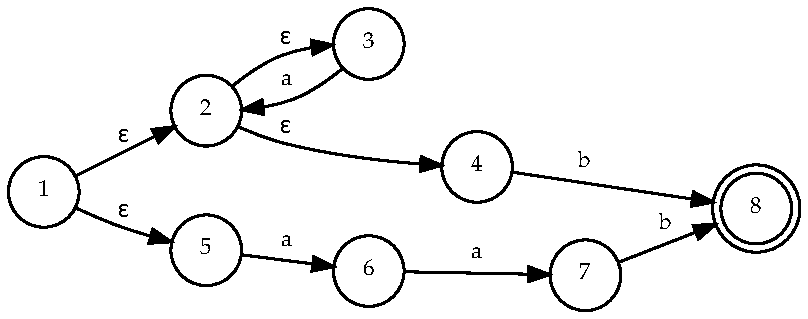
\includegraphics[width=\textwidth]{matching/ex_matching.pdf}
    \caption{NFA for the regular expression \textsf{a*b\textbar aab}}
    \label{fig:ex_matching}
  \end{figure}
  
  In this example we will demonstrate how the regular expression
  \textsf{a*b\textbar aab} is matched with the string \textsl{aab}. In
  figure \vref{fig:ex_matching} we have the corresponding NFA. Each
  state is marked with a unique number which we will be referring to
  in the table below.

\begin{center}
\begin{tabular}{ccp{8.5cm}}
Active set & \texttt{SP} & Explanation \\
\hline

1 & \textsl{\underline{a}ab} & Initially we have the start state in
the active set and \texttt{SP} points to the start of the string. \\

3, 4, 5 & \textsl{\underline{a}ab} & Following all
$\upvarepsilon$-transitions. \\

2, 6 & \textsl{a\underline{a}b} & Reading the first \textsl{a} from the input
string, states 3 and 5 have legal transitions on \textsl{a}. \\

3, 4, 6 & \textsl{a\underline{a}b} & Following all
$\upvarepsilon$-transitions. \\

2, 7 & \textsl{aa\underline{b}} & Reading the second \textsl{a} from
the input string, states 3 and 6 have legal transitions on
\textsl{a}. \\

3, 4, 6 & \textsl{aa\underline{b}} & Following all
$\upvarepsilon$-transitions. \\

8 & \textsl{aab\underline{ }} & Reading the last character from input
string: \textsl{b}, states 4 and 7 have legal transitions on
\textsl{b}. \\

8 & \textsl{aab\underline{ }} & No $\upvarepsilon$-transitions to follow.

\end{tabular}
\end{center}

After reading the string we can see that the accepting state is in the
active set: We have a match!

\end{example}


\subsection{Protocol specification}
\label{sec:protocol_spec}

In this section we will define a protocol that can communicate
information between our processes. The information consists of the
mixed bit-values generated by the NFA simulator and the filters. The
protocol should enable us to recreate paths taken through an NFA. To
this purpose we need the protocol to support the following operators:

\begin{description}
  \item[\textbar] The end of the channel list is reached and we should
    set the active channel to the first channel. This coincides with
    reading a new character. It is not a strictly necessary operator,
    we can make do with the change channels action. We choose to keep
    a separate action for end of list, because it adds to readability
    and redundancy.
  \item[:] Whenever we change channels we put a :. There may be more
    than one or perhaps even no bits output on a channel for any given
    character from the string
  \item[=] Copying of a channel. One channel is split into two, the
    paths taken through the NFA will be identical up to the point of
    splitting. The newly created channel is put in front of the rest
    of the channels
  \item[0,1, \textbackslash $a$] The actual bit values. The character
    classes needs extra care, we need to know on which character we
    passed them, so we put the value we pass on, escaped in the output
  \item[b] A channel is abandoned with no match
  \item[t] A channel has a match
\end{description}

\begin{example}[Protocol]
  In figure \vref{fig:ex_prot} we have an automaton for regular
  expression \textsf{a*}. When matching this regular expression with
  the string \textsl{aa} we generate some mixed bit-values. This
  example will in detail demonstrate how the mixed bit-values are
  generated.
  \begin{figure}
    \centering
    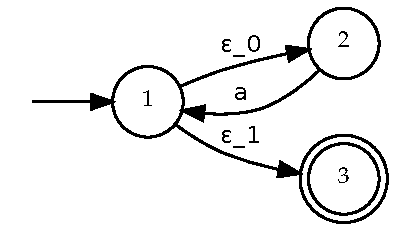
\includegraphics{matching/example_protocol.pdf}
    \caption{Automaton with bitvalues for regular expression
      \texttt{a*}}
    \label{fig:ex_prot}
  \end{figure}
  
  \begin{description}
  
  \item[Initial step:] Initially the start state of the automaton is
    added to the active list. All $\upvarepsilon$-edges are followed
    and the following is output:
    \begin{enumerate}
    \item Node 1 is a split-node, a \texttt{=} is output, and we
      follow the $\upvarepsilon$-edge to node 2 and output a
      \texttt{0}. We can not make any further progress on this
      channel. We output a \texttt{:} and switch to the next channel.

      Output so far: \texttt{=0:}. \\
      List of active channels: $\{2, 1\}$.
    \item The active channel is now in node 1, we follow the
      $\upvarepsilon$-edge from node 1 to 3 and output a
      \texttt{1}. We can not make any further progress on this
      channel. This is the last channel in the channel list, so we
      output a \texttt{|} and reset the active channel.

      Output so far: \texttt{=0:1|}.\\
      List of active channels: $\{2, 3\}$.
    \end{enumerate}

  \item[First \textsl{a} is read]
    \begin{enumerate}
    \item Node 2 has a transition marked \texttt{a}, we follow this
      back to node 1. Node 1 is a split-node, a \texttt{=} is output,
      and we follow the $\upvarepsilon$-edge to node 2 and output a
      \texttt{0}. We can not make any further progress on this
      channel. We output a \texttt{:} and switch to the next channel.

      Output so far: \texttt{=0:1|=0:}. \\
      List of active channels: $\{2, 1, 3\}$.
    \item The active channel is now in node 1, we follow the
      $\upvarepsilon$-edge from node 1 to 3 and output a
      \texttt{1}. We can not make any further progress on this
      channel. We output a \texttt{:} and switch to the next channel.

      Output so far: \texttt{=0:1|=0:1:}. \\
      List of active channels: $\{2, 3, 3\}$.
    \item Node 3 is the accepting node and does not have any
      transitions. We abandon this channel and output a
      \texttt{b}. This is the last channel in the channel list, so we
      output a \texttt{|} and reset the active channel.

      Output so far: \texttt{=0:1|=0:1:b|}. \\
      List of active channels: $\{2, 3\}$.
    \end{enumerate}
  \item[Second \textsl{a} is read] This is the final step.
    \begin{enumerate}
      \item From node 2 we can make a transition on \texttt{a} back to
        node 1. This is a split node, so we output a \texttt{=} and
        transition on the the $\upvarepsilon$-edge to node 2 and
        output a \texttt{0}. We can not do further transitions and
        this is not the accepting node, we abandon this channel and
        output a \texttt{b}. We switch to the next channel and output
        a \texttt{:}.

        Output so far: \texttt{=0:1|=0:1:b|=0b:}. \\
        List of active channels: $\{1, 3\}$.
      \item Node 1 has a $\upvarepsilon$-transition to node 3, we take
        it and output a \texttt{1}. We can not do further transitions
        and since this is the accepting node, we output a
        \texttt{t}. We have one channel left, so we output a
        \texttt{:} and switch.

        Output so far: \texttt{=0:1|=0:1:b|=0b:1t:}. \\
        List of active channels: $\{3\}$.
      \item Node 3 has no available transitions. We abandon this
        channel and output a \texttt{b}.

        Output so far: \texttt{=0:1|=0:1:b|=0b:1t:b}. \\
        List of active channels: $\{\}$.
    \end{enumerate}
  \end{description}
\end{example}

